%versi 3 (22-07-2020)
\chapter{Landasan Teori}
\label{chap:teori}
Bab ini akan membahas dasar-dasar teori dalam pengembangan perangkat lunak KIRI. Pembahasan akan dimulai dari perangkat lunak KIRI, \textit{design pattern} dan \textit{strategy pattern} beserta conton kode penerapan \textit{strategy pattern}, MySQL beserta pembahasan mengenai \textit{LineString}, penjelasan mengenai graf termasuk graf berarah dan graf tidak berarah serta graf berbobot dan graf tidak berbobot, dan algoritma \textit{shortest path} yang didalamnya akan dijelaskan juga algoritma-algoritma \textit{shortest path} yang diimplementasikan, yaitu Dijkstra, Floyd-Warshall, dan A-Star.
\section{KIRI ~\cite{nugroho_natali:17:KIRI}}
\label{sec:kiri}
KIRI (lihat Gambar \ref{fig:tampilanawalkiri}) adalah aplikasi navigasi transportasi umum berbasis web yang menyediakan rute antara dua lokasi geografis menggunakan transportasi publik. KIRI dirancang untuk melayani kebutuhan pengguna angkot (angkutan kota) di Bandung serta TransJakarta dan Commuterline di DKI Jakarta. Salah satu keunggulan KIRI dibandingkan layanan seperti Google Maps atau Moovit adalah kemampuannya memahami karakteristik  transportasi publik, di mana penumpang dapat naik atau turun di sepanjang jalan tanpa terbatas pada halte tertentu.
\begin{figure}[H] 
	\centering  
	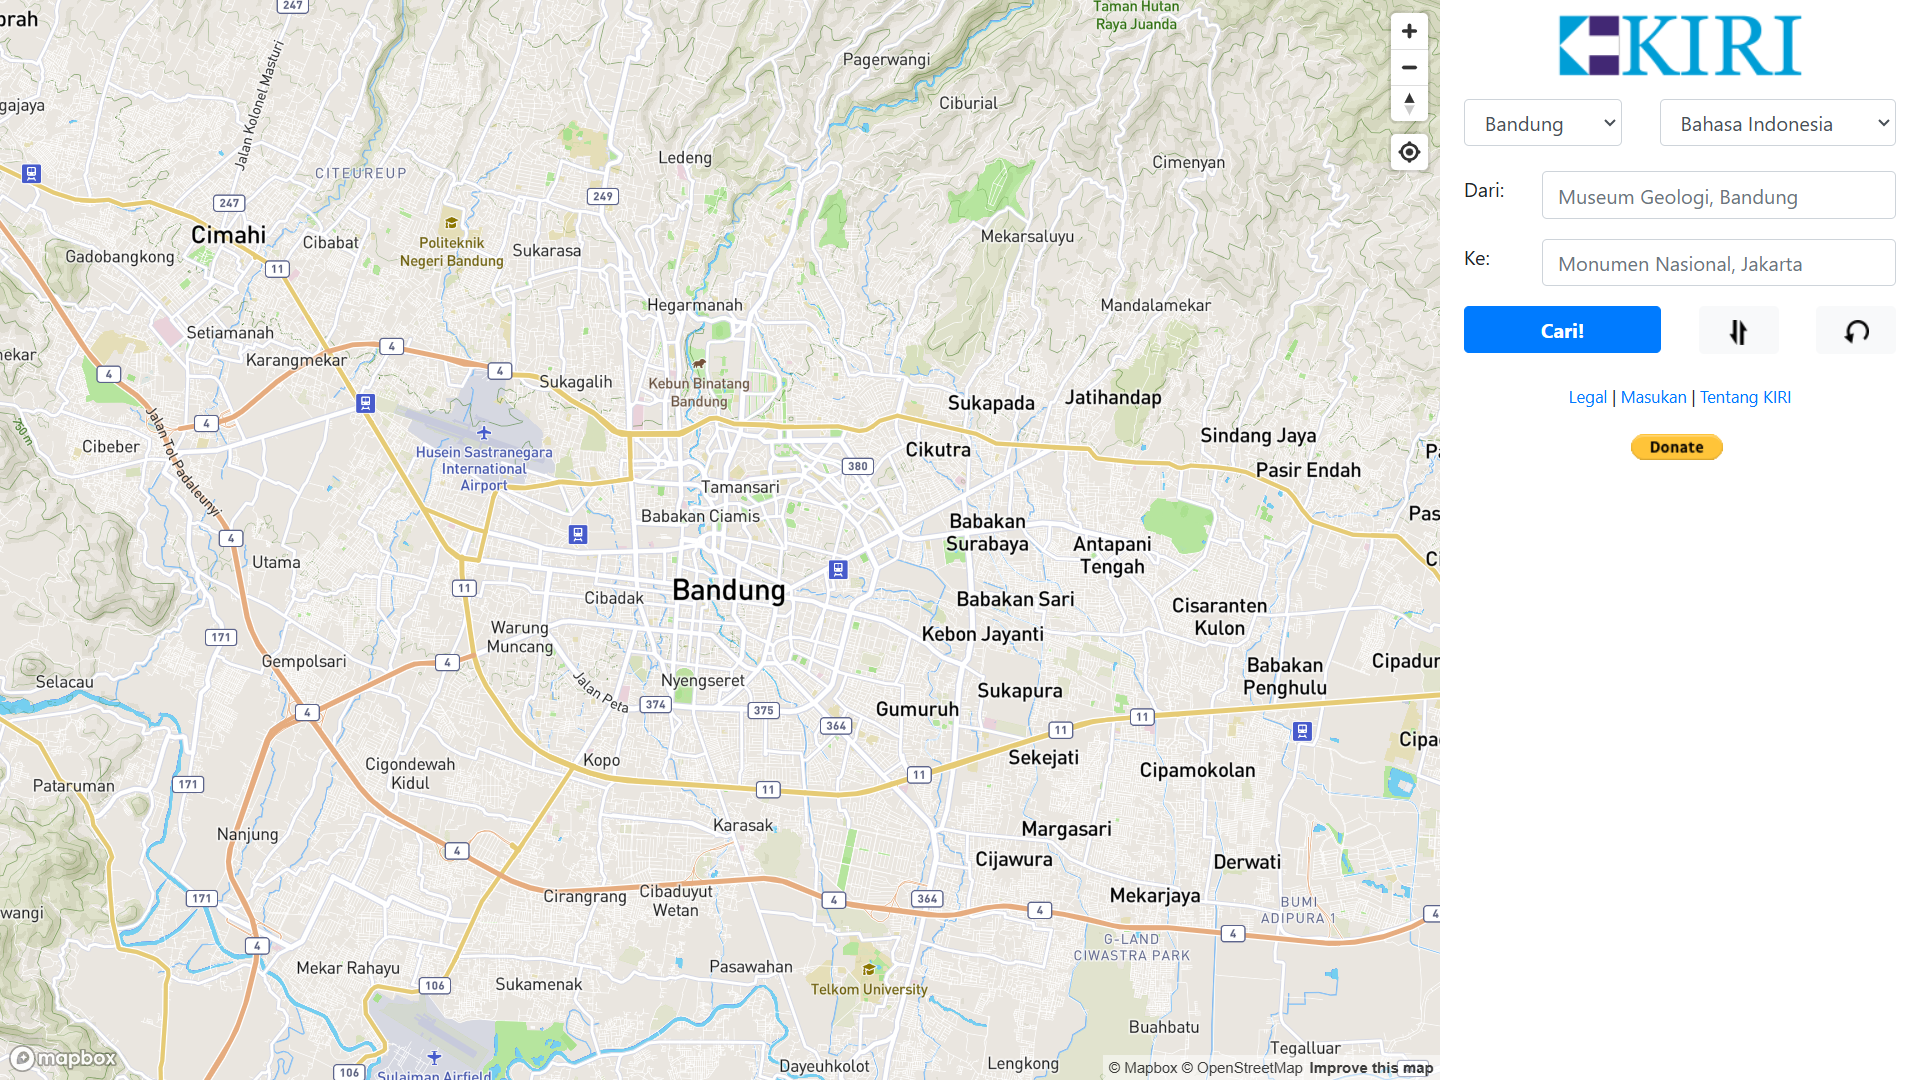
\includegraphics[width=0.9\textwidth]{KIRI}  
	\caption{Tampilan awal perangkat lunak KIRI}
	\label{fig:tampilanawalkiri} 
\end{figure}
\newpage
KIRI akan memberikan informasi mengenai langkah-langkah yang harus ditempuh oleh pengguna yang akan berpergian dari satu tempat ke tempat tujuannya, mulai dari seberapa jauh pengguna harus berjalan untuk menaiki angkot yang bersangkutan, di mana pengguna harus naik atau turun angkot tersebut, seberapa jauh lagi pengguna harus berjalan sampai ke lokasi tujuan, dan seberapa lama estimasi waktu perjalanan yang akan ditempuh (lihat Gambar \ref{fig:tampilankiri}).
\begin{figure}[H] 
	\centering  
	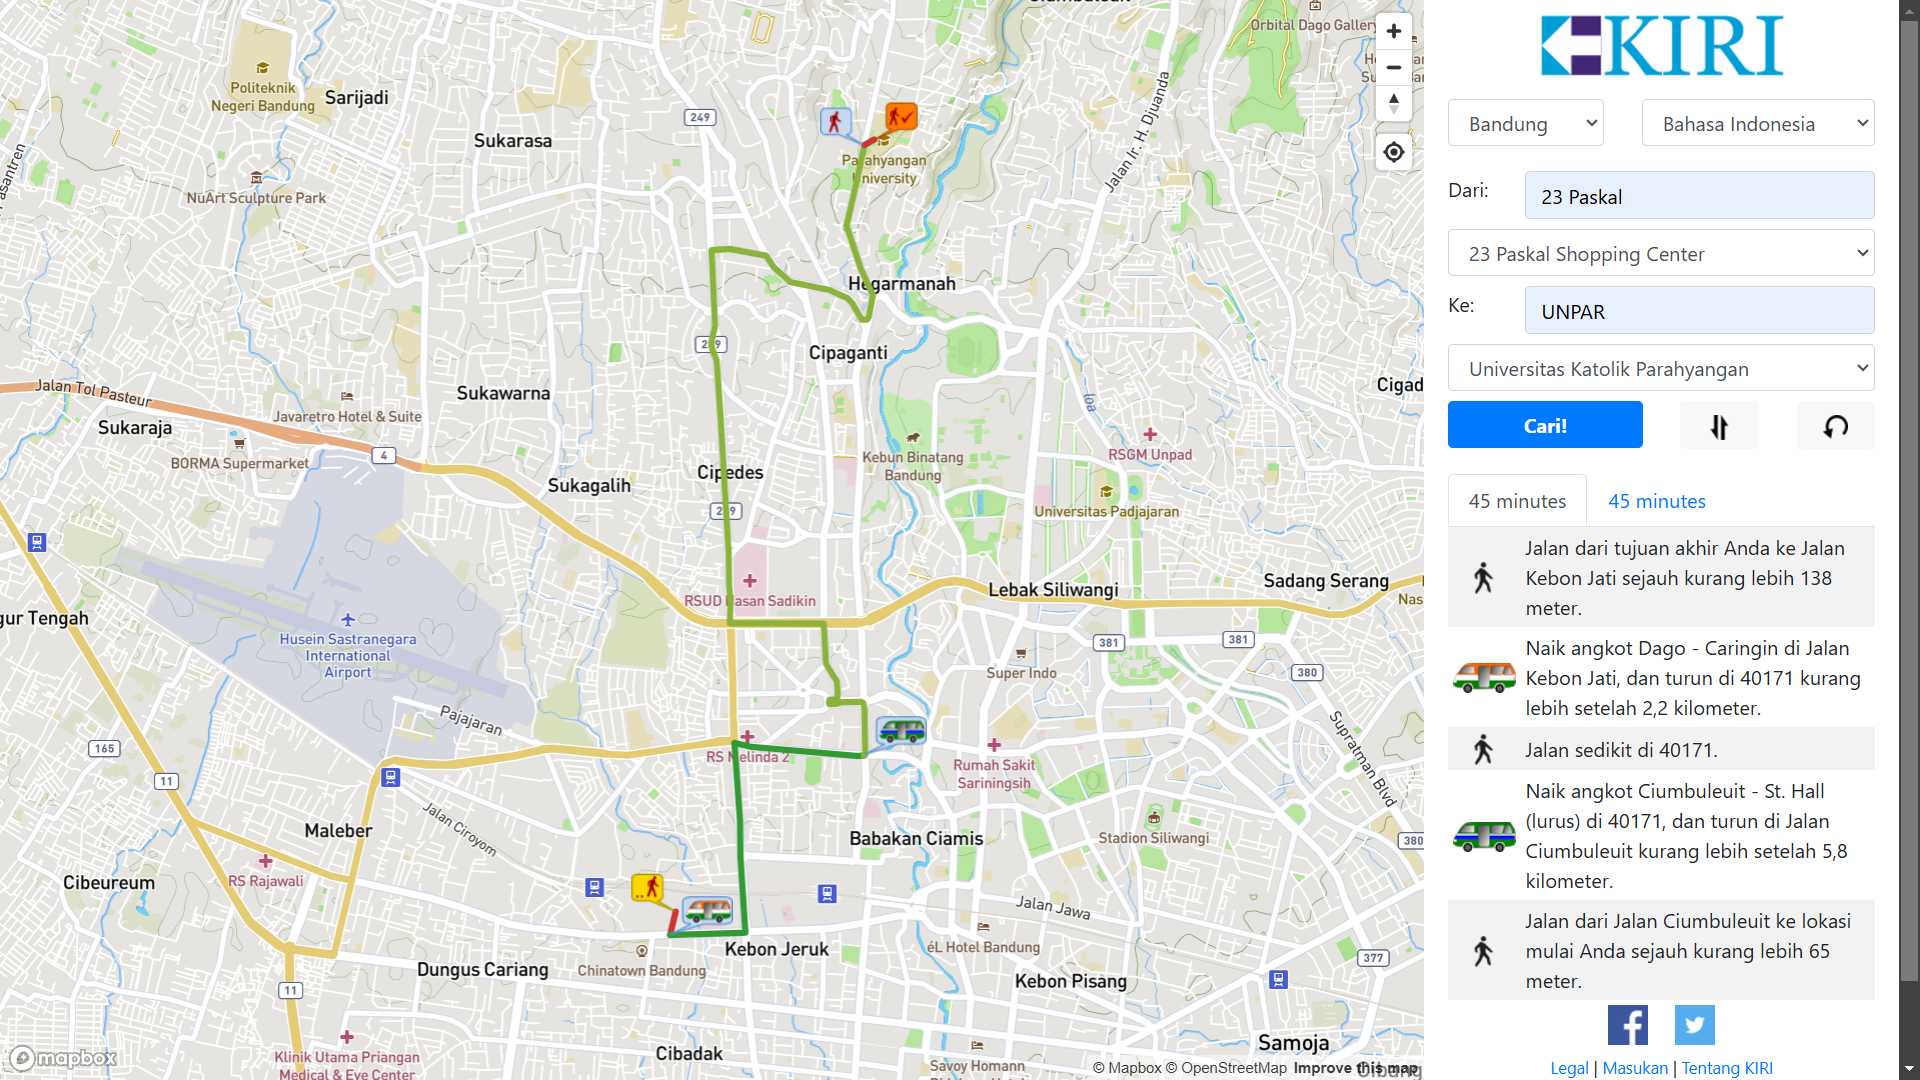
\includegraphics[width=1\textwidth]{KIRI-2}  
	\caption{Tampilan perangkat lunak KIRI, setelah menerima masukan}
	\label{fig:tampilankiri} 
\end{figure}

Arsitektur aplikasi KIRI terbagi menjadi dua bagian utama. Yang pertama, yaitu Tirtayasa yang merupakan bagian \textit{frontend} dari KIRI, dan bertanggung jawab sebagai antarmuka pengguna untuk browser web. Komponen ini mengubah nama tempat yang dimasukkan pengguna menjadi koordinat geografis dengan menggunakan bantuan Google Maps. Tirtayasa sendiri dibangun menggunakan PHP dan \textit{framework} CodeIgniter 3.

Selanjutnya, NewMenjangan, yang merupakan bagian \textit{backend} dari KIRI dan dibangun dengan bahasa pemrogrman Java serta digunakan untuk memproses permintaan navigasi. Komponen ini memuat semua jalur transportasi umum dalam bentuk graf dan menggunakan algoritma Dijkstra untuk menghitung rute optimal. Algoritma ini dipercepat dengan penggunaan struktur data heap, yang membuatnya efisien untuk jalur yang kompleks.

\section{Design Pattern dan Strategy Pattern ~\cite{Gamma:94:design}}
\label{sec:designdanstrategypattern}
\textit{Design Pattern} adalah sebuah solusi untuk mengatasi masalah desain berulang dalam pengembangan perangkat lunak berorientasi objek. Solusi ini dirancang agar dapat digunakan kembali di berbagai konteks tanpa harus disesuaikan secara berlebihan. Sebagai contoh, \textit{design Pattern} membantu memecah masalah desain menjadi struktur yang lebih modular dan fleksibel, sehingga mempermudah pengembangan dan pemeliharaan perangkat lunak.

Pada dasarnya, \textit{design pattern} memiliki empat elemen utama. Elemen-elemen tersebut diantaranya, yaitu, yang pertama adalah nama pola yang memberikan cara singkat untuk menyebut masalah desain tertentu. Kedua, masalah, yaitu deskripsi konteks atau situasi di mana \textit{design pattern} ini relevan. Ketiga, solusi yang berupa abstraksi dari elemen-elemen desain dan kolaborasinya tanpa menyebutkan implementasi konkret. Keempat, konsekuensi yang mencakup hasil dari penerapan pola, termasuk dampak pada fleksibilitas, efisiensi, dan pengelolaan sistem.

Penggunaan \textit{design pattern} juga memungkinkan sistem menjadi lebih adaptif terhadap perubahan kebutuhan. Pola seperti \textit{Strategy} atau \textit{strategy pattern} mempermudah pergantian algoritma di \textit{runtime}, sedangkan \textit{Factory Method} membantu mengurangi ketergantungan pada implementasi spesifik dengan menyediakan cara fleksibel untuk membuat objek. Dengan demikian, \textit{design pattern} mempermudah kolaborasi dan komunikasi antar tim pengembang.

\textit{Strategy pattern} merupakan salah satu pola desain perilaku yang dirancang untuk mendefinisikan serangkaian algoritma, mengenkapsulasi setiap algoritma, dan memungkinkan algoritma-algoritma tersebut untuk saling dipertukarkan. Pola ini memungkinkan algoritma untuk bervariasi. Dengan demikian, klien tidak perlu mengetahui detail implementasi dari algoritma yang digunakan, melainkan cukup berinteraksi melalui antarmuka umum yang disediakan oleh objek strategi.

Pola ini sangat berguna ketika terdapat kebutuhan untuk mendukung berbagai varian algoritma dalam menyelesaikan tugas yang sama. \textit{Strategy pattern} memindahkan setiap algoritma ke dalam kelas terpisah, yang disebut sebagai \textit{concrete strategy}. Sistem dapat memilih dan menentukan strategi yang sesuai ke dalam konteks pada waktu eksekusi, sehingga memberikan fleksibilitas yang tinggi dalam proses pengembangan perangkat lunak.

Manfaat utama dari \textit{strategy pattern} adalah kemampuannya untuk menghilangkan kompleksitas yang diakibatkan oleh penggunaan pernyataan kondisional yang rumit dalam kode, serta kemudahan dalam menambahkan atau mengganti algoritma tanpa perlu memodifikasi kode klien atau konteks. Namun, penerapan pola ini juga memiliki kelemahan, seperti meningkatnya jumlah kelas dalam sistem dan potensi timbulnya \textit{overhead} komunikasi antara konteks dan strategi. Oleh karena itu, penerapan \textit{strategy pattern} sebaiknya dipertimbangkan dengan cermat, terutama dalam situasi di mana variasi algoritma memang diperlukan untuk memenuhi kebutuhan sistem.
\\
Berikut merupakan struktur dari strategy pattern (Gambar \ref{fig:struktursp}).
\begin{figure}[h] 
	\centering  
	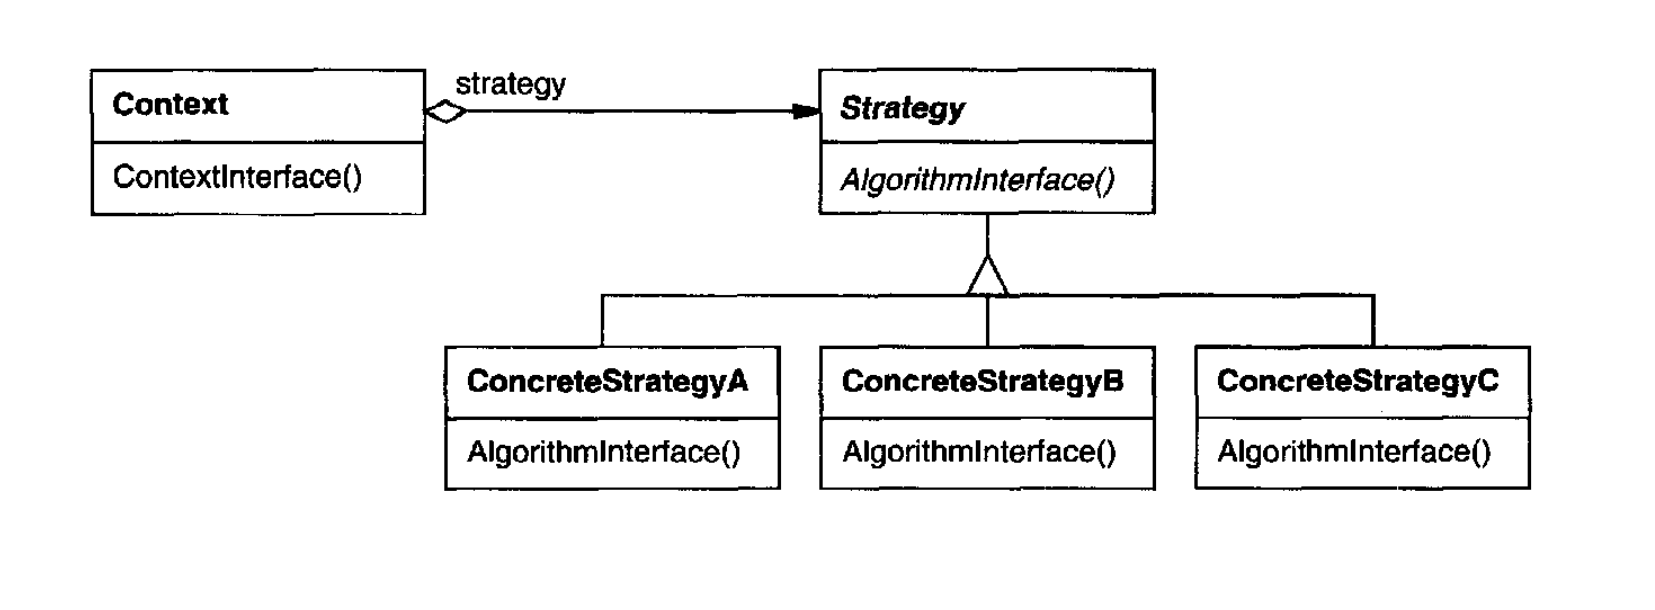
\includegraphics[width=1\textwidth]{struktur-sp}  
	\caption{Struktur Strategy Pattern}
	\label{fig:struktursp} 
\end{figure}
\newpage
\subsection{Contoh Kode Program}
\label{sec:kode}
\begin{lstlisting}[language=Java, caption=IntegerSorter.java, basicstyle=\small\ttfamily]
    abstract class IntegerSorter {
        public abstract int[] sort(int[] arr);
    }
\end{lstlisting}

\begin{lstlisting}[language=Java, caption=ArraysSort.java, basicstyle=\small\ttfamily]
    import java.util.*;

    class ArraysSort extends IntegerSorter {
        public int[] sort(int[] arr) {
            Arrays.sort(arr);
            return arr;
        }
    }
\end{lstlisting}

\begin{lstlisting}[language=Java, caption=BubbleSort.java, basicstyle=\small\ttfamily]
    class BubbleSort extends IntegerSorter {
        public int[] sort(int[] arr) {
            int n = arr.length;
            for (int i = 0; i < n - 1; i++) {
                for (int j = 0; j < n - i - 1; j++) {
                    if (arr[j] > arr[j + 1]) {
                        int temp = arr[j];
                        arr[j] = arr[j + 1];
                        arr[j + 1] = temp;
                    }
                }
            }
            return arr;
        }
    }
\end{lstlisting}

\begin{lstlisting}[language=Java, caption=InsertionSort.java, basicstyle=\small\ttfamily]
    class InsertionSort extends IntegerSorter {
        public int[] sort(int[] arr) {
            int n = arr.length;
            for (int i = 1; i < n; i++) {
                int key = arr[i];
                int j = i - 1;
    
                while (j >= 0 && arr[j] > key) {
                    arr[j + 1] = arr[j];
                    j = j - 1;
                }
                arr[j + 1] = key;
            }
            return arr;
        }
    }
\end{lstlisting}

\begin{lstlisting}[language=Java, caption=Main.java, basicstyle=\small\ttfamily]
    import java.util.*;

    public class Main {
        public static void main(String[] args) {
            int[] arr = { 6, 4, 21, 9, 14, 17, 3 };
    
            IntegerSorter arraysSort = new ArraysSort();
            System.out.println("Arrays.sort: " + Arrays.toString(arraysSort.sort(arr.clone())));
    
            IntegerSorter bubbleSort = new BubbleSort();
            System.out.println("Bubble Sort: " + Arrays.toString(bubbleSort.sort(arr.clone())));
    
            IntegerSorter insertionSort = new InsertionSort();
            System.out.println("Insertion Sort: " + Arrays.toString(insertionSort.sort(arr.clone())));
    
        }
    }
\end{lstlisting}


\section{MySQL ~\cite{oracle:24:mysql8.4}}
\label{sec:mysql}
MySQL merupakan sistem manajemen basis data relasional (\textit{Relational Database Management System}/RDBMS) bersifat \textit{open source} yang dikembangkan oleh Oracle Corporation. SQL, yang merupakan singkatan dari \textit{Structured Query Language}, adalah bahasa pemrograman yang digunakan untuk mengambil, memperbarui, menghapus, serta memanipulasi data pada basis data relasional.

Sebagai basis data relasional, MySQL menyimpan data dalam bentuk tabel yang terdiri atas baris dan kolom, yang disusun dalam suatu skema. Skema ini bertugas mendefinisikan bagaimana data diorganisasi dan disimpan, serta menjelaskan hubungan antara tabel-tabel yang ada di dalamnya.

Dalam MySQL, terdapat berbagai sintaks yang digunakan untuk mendukung pengelolaan basis data. Sintaks-sintaks tersebut mencakup operasi penting, seperti pembuatan tabel, penyisipan data, pembaruan data, penghapusan data, hingga pengambilan data. Setiap sintaks dirancang untuk mempermudah pengguna dalam mengelola data secara efektif dan efisien sesuai kebutuhan sistem. Berikut merupakan sintaks-sintaks dasar yang umum digunakan dalam MySQL.
\begin{itemize}
    \item \textbf{\textit{CREATE DATABASE}}
    \begin{lstlisting}[language=SQL]
    CREATE DATABASE database_name;
    \end{lstlisting}
    Sintaks tersebut digunakan untuk membuat database baru dalam MySQL. \texttt{database\_name} diisi nama dari database baru yang akan dibuat.
    \item \textbf{\textit{DROP DATABASE}}
    \begin{lstlisting}[language=SQL]
    DROP DATABASE database_name;
    \end{lstlisting}
    Sintaks tersebut digunakan untuk menghapus database yang telah dibuat dalam MySQL. \texttt{database\_name} diisi nama dari database yang akan dihapus.
    
    \item \textbf{\textit{CREATE TABLE}}
    \begin{lstlisting}[language=SQL]
    CREATE TABLE table_name (
        column1 datatype,
        column2 datatype,
        column3 datatype,
        ....
    );
    \end{lstlisting}
    Sintaks tersebut digunakan untuk membuat atau memasukan tabel baru kedalam sebuah database. \texttt{table\_name} diisi nama dari tabel yang akan dibuat, \texttt{column1, column2, column3} dan seterusnya diisi dengan nama kolom didalam tabel yang akan dibuat, dan \texttt{datatype} diisi dengan tipe data dari kolom yang akan dibuat, seperti \texttt{varchar}, \texttt{integer}, \texttt{date}, dan lain-lain.

    \item \textbf{\textit{DROP TABLE}}
    \begin{lstlisting}[language=SQL]
    DROP TABLE table_name;;
    \end{lstlisting}
    Sintaks tersebut digunakan untuk menghapus tabel yang telah dibuat dalam sebuah database. \texttt{table\_name} diisi nama dari tabel yang akan dihapus.

    \item \textbf{\textit{SELECT}}
    \begin{lstlisting}[language=SQL]
    SELECT column1, column2, ...
    FROM table_name;
    \end{lstlisting}
    Sintaks tersebut digunakan untuk memilih atau mengambil data dari sebuah tabel dalam database. \texttt{column1, column2} dan seterusnya diisi dengan nama kolom dari sebuah tabel yang datanya akan diambil dan \texttt{table\_name} diisi dengan nama tabel kolom tersebut berada.

    \item \textbf{\textit{WHERE}}
    \begin{lstlisting}[language=SQL]
    SELECT column1, column2, ...
    FROM table_name
    WHERE condition;
    \end{lstlisting}
    Sintaks tersebut digunakan untuk memilih atau mengambil data dari sebuah tabel dalam database dengan sebuah kondisi tertentu yang bertujuan untuk memfilter data yang akan diambil. \texttt{column1, column2} dan seterusnya diisi dengan nama kolom dari sebuah tabel yang datanya akan diambil, \texttt{table\_name} diisi dengan nama tabel di mana kolom tersebut berada, dan \texttt{condition} diisi dengan kondisi dari data yang akan diambil atau filter seperti apa yang ingin dilakukan ketika mengambil data.

    \item \textbf{\textit{INSERT INTO}}
    \begin{lstlisting}[language=SQL]
    INSERT INTO table_name (column1, column2, column3, ...)
    VALUES (value1, value2, value3, ...);
    \end{lstlisting}
    Sintaks tersebut digunakan untuk menambahkan data baru kedalam kolom dari sebuah tabel yang telah ada. \texttt{tabel\_name} diisi nama tabel yang akan ditambahkan data baru, \texttt{column1, column2, column3} dan seterusnya diisi dengan nama kolom yang akan ditambahkan data baru, dan \texttt{value} diisi dengan nilai atau \textit{value} dari data baru yang akan ditambahkan.

    \item \textbf{\textit{DELETE}}
    \begin{lstlisting}[language=SQL]
    DELETE FROM table_name
    WHERE condition;
    \end{lstlisting}
     Sintaks tersebut digunakan untuk menghapus data dari sebuah tabel dengan kondisi tertentu. \texttt{tabel\_name} diisi nama tabel yang datanya akan dihapus, dan \texttt{condition} diisi dengan kondisi data dari yang akan dihapus filter seperti apa yang ingin dilakukan ketika menghapus data.
\end{itemize}

\subsection{LineString ~\cite{oracle:24:mysql8.4}}
\label{subs:linestring}
\textit{LineString} adalah tipe data geometris dalam MySQL yang mewakili jalur atau lintasan yang terdiri dari satu atau lebih segmen garis yang terhubung. Tipe data ini digunakan dalam Sistem Informasi Geografis atau \textit{Geographic Information System} (GIS) untuk merepresentasikan lintasan seperti jalan, sungai, atau rute perjalanan. Setiap \textit{LineString} terdiri dari urutan titik (\textit{point}) yang memiliki koordinat (x, y) dan minimal memiliki dua titik untuk membentuk garis.

Untuk memanipulasi dan menganalisis \textit{LineString}, MySQL menyediakan sejumlah fungsi bawaan. Sebelum fungsi tersebut digunakan, objek \textit{LineString} biasanya dikonversi ke bentuk geometris menggunakan fungsi \texttt{ST\_GeomFromText()}. Fungsi ini menerima teks representasi geometris, seperti $LineString(x1 y1, x2 y2, ...)$ dan mengubahnya menjadi objek geometris yang dapat diproses oleh fungsi lainnya. Berikut adalah beberapa fungsi dalam \textit{LineString}:
\begin{itemize}
    \item \texttt{ST\_EndPoint(ls)}
    \\ Mengembalikan titik akhir dari \textit{LineString} $ls$. Contoh:
    \begin{lstlisting}[language=SQL]
    SET @ls = 'LineString(1 1, 2 2, 3 3)';
    SELECT ST_AsText(ST_EndPoint(ST_GeomFromText(@ls))); 
    -- Hasil: 'POINT(3 3)'
    \end{lstlisting}
    
    \item \texttt{ST\_IsClosed(ls)}
    \\ Mengecek apakah \textit{LineString} $ls$ membentuk lintasan tertutup (titik awal dan akhir sama). Contoh: 
    \begin{lstlisting}[language=SQL]
    SET @ls = 'LineString(1 1, 2 2, 3 3, 1 1)';
    SELECT ST_IsClosed(ST_GeomFromText(@ls));
    -- Hasil: 1 (TRUE)
    \end{lstlisting}
    
    \item \texttt{ST\_Length(ls)}
    \\ Menghitung panjang total \textit{LineString} $ls$. Contoh: \begin{lstlisting}[language=SQL]
    SET @ls = 'LineString(1 1, 2 2, 3 3)';
    SELECT ST_Length(ST_GeomFromText(@ls));
    -- Hasil: 2.828427
    \end{lstlisting}

    \item \texttt{ST\_NumPoints(ls)}
    \\ Mengembalikan jumlah titik yang membentuk \textit{LineString} $ls$. Contoh: 
    \begin{lstlisting}[language=SQL]
    SET @ls = 'LineString(1 1, 2 2, 3 3)';
    SELECT ST_NumPoints(ST_GeomFromText(@ls));
    -- Hasil: 3
    \end{lstlisting}
    
    \item \texttt{ST\_Point(ls, N)}
    \\ Mengembalikan titik ke-$N$ pada \textit{LineString} $ls$. Contoh: \begin{lstlisting}[language=SQL]
    SET @ls = 'LineString(1 1, 2 2, 3 3)';
    SELECT ST_AsText(ST_PointN(ST_GeomFromText(@ls), 2));
    -- Hasil: 'POINT(2 2)'
    \end{lstlisting}
    
    \item \texttt{ST\_StartPoint(ls)}
    \\ Mengembalikan titik awal dari \textit{LineString} $ls$. Contoh: \begin{lstlisting}[language=SQL]
    SET @ls = 'LineString(1 1, 2 2, 3 3)';
    SELECT ST_AsText(ST_StartPoint(ST_GeomFromText(@ls)));
    -- Hasil: 'POINT(1 1)'
    \end{lstlisting}

\end{itemize}

\section{Graf ~\cite{Diestel:17:graph}}
\label{sec:graph}
Graf ($G$) adalah struktur yang terdiri dari simpul (\textit{vertex}) dan sisi (\textit{edge}), di mana sisi menghubungkan pasangan simpul (lihat Gambar \ref{fig:graf}). Sebuah graf direpresentasikan sebagai pasangan $G=(V,E)$, dengan $V$ sebagai himpunan simpul dan $E$ sebagai himpunan sisi. Sisi diwakili oleh pasangan simpul yang terhubung. Graf dapat bersifat berarah atau tidak berarah dan juga berbobot atau tidak berbobot. Graf digunakan dalam berbagai hal, seperti jaringan komputer, rute transportasi, dan analisis hubungan sosial.
\begin{figure}[H] 
    \centering  
    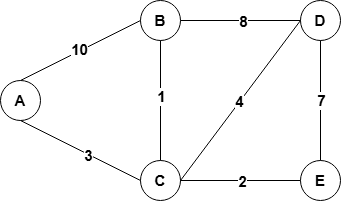
\includegraphics[width=0.65\textwidth]{graf-kasus}  
    \caption{Graf}
    \label{fig:graf} 
\end{figure}

Simpul-simpul dalam graf dapat memiliki derajat tertentu, yaitu jumlah sisi yang menghubungkannya. Sebuah graf disebut terhubung jika terdapat jalur antara setiap pasangan simpul. Jalur ini adalah urutan simpul yang dihubungkan oleh sisi. Teori graf juga mencakup konsep seperti pohon (graf terhubung tanpa siklus), graf bipartit (simpul dibagi menjadi dua himpunan yang saling bebas sisi), dan subgraf (bagian dari graf yang tetap mempertahankan struktur graf).

\subsection{Graf Berarah dan Graf Tidak Berarah~\cite{Diestel:17:graph}}
\label{sec:grafberarah}
Graf berarah (lihat Gambar \ref{fig:grafberarah}) adalah graf yang di mana setiap sisi memiliki arah tertentu. Dengan kata lain, setiap sisi dalam graf ini diwakili oleh pasangan terurut dari simpul (\textit{vertex}). Sebuah graf berarah didefinisikan sebagai pasangan $G=(V,E)$, di mana $V$ adalah himpunan simpul dan $E$ adalah himpunan sisi yang berbentuk pasangan terurut dari simpul. Setiap sisi $e$ memiliki simpul awal dan simpul terminal yang menunjukkan arah perjalanan dari satu simpul ke simpul lainnya.

Graf berarah dapat memiliki berbagai karakteristik khusus yang membedakannya dari graf tidak berarah. Jika terdapat lebih dari satu sisi dengan arah yang sama antara dua simpul yang sama, sisi tersebut disebut sisi paralel. Jika sebuah sisi memiliki awal dan terminal yang sama, maka sisi tersebut disebut loop. Selain itu, Jika suatu graf tidak berarah diberikan arah pada setiap sisinya, maka graf berarah yang dihasilkan disebut sebagai \textit{oriented graph}.

\begin{figure}[H] 
    \centering  
    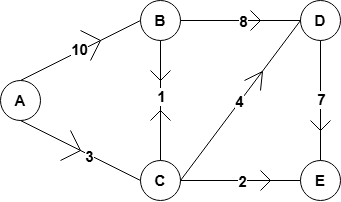
\includegraphics[width=0.7\textwidth]{graf-berarah}  
    \caption{Graf Berarah}
    \label{fig:grafberarah} 
\end{figure}

Graf tidak berarah (lihat Gambar \ref{fig:graf}) adalah jenis graf di mana setiap sisi hanya menghubungkan dua simpul tanpa adanya arah tertentu. Dalam graf ini, sisi diwakili sebagai pasangan tidak terurut \{$u,v$\} yang berarti bahwa pergerakan dari simpul $u$ ke $v$ sama dengan pergerakan dari $v$ ke $u$. Graf tidak berarah dapat direpresentasikan dalam bentuk matriks ketetanggaan (\textit{adjacency matrix}), di mana matriks ini bersifat simetris.

Salah satu sifat penting dari graf tidak berarah adalah konsep keterhubungan. Sebuah graf dikatakan terhubung jika terdapat jalur antara setiap pasangan simpulnya. Jika terdapat simpul yang tidak dapat dijangkau dari simpul lain, maka graf tersebut disebut tidak terhubung. Selain keterhubungan, graf tidak berarah juga memiliki properti siklus, yaitu jalur tertutup di mana simpul awal dan simpul akhir adalah sama.

\subsection{Graf Berbobot dan Graf Tidak Berbobot ~\cite{Diestel:17:graph}}
\label{sec:grafberbobot}
Graf berbobot (\textit{weighted graph}) (lihat Gambar \ref{fig:graf}) adalah graf di mana setiap sisi memiliki bobot atau nilai numerik yang menyatakan karakteristik tertentu seperti jarak, biaya, atau kapasitas. Graf berbobot direpresentasikan sebagai $G = (V,E,w)$, di mana $w:E\rightarrow R$ adalah fungsi yang memberikan bobot pada setiap sisi.

Graf berbobot sering digunakan dalam berbagai aplikasi seperti  algoritma pencarian jalur terpendek, optimasi jaringan, serta pemodelan sistem transportasi. Dalam beberapa kasus, graf berbobot dapat bersifat berarah jika bobot hanya berlaku dalam satu arah antara dua simpul, atau tidak berarah jika bobot berlaku dua arah secara simetris antara kedua simpul yang terhubung.
\newpage
\begin{figure}[H] 
    \centering  
    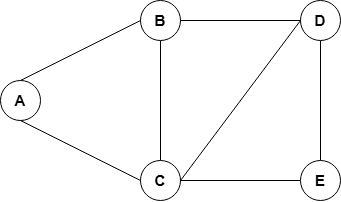
\includegraphics[width=0.7\textwidth]{graf-tidak-berbobot}  
    \caption{Graf Tidak Berbobot}
    \label{fig:graftidakberbobot} 
\end{figure}
Graf tidak berbobot (lihat Gambar \ref{fig:graftidakberbobot}) adalah graf di mana semua sisi dianggap memiliki bobot yang sama, biasanya bernilai satu atau dianggap tidak berbobot sama sekali. Graf jenis ini sering digunakan dalam analisis struktur jaringan, di mana hanya penting untuk mengetahui adanya hubungan antar simpul tanpa mempertimbangkan seberapa kuat atau penting hubungan tersebut.

Dalam graf tak berbobot, algoritma seperti BFS (Breadth-First Search) dan DFS (Depth-First Search) sangat berguna untuk menemukan keterhubungan, jalur terpendek dalam jumlah langkah, serta untuk eksplorasi struktur graf lainnya.



\section{Algoritma Shortest Path}
\label{sec:algoritmasp}
Terdapat berbagai jenis algoritma shortest path yang dirancang untuk menentukan lintasan terpendek antara dua simpul dalam suatu graf. Algoritma-algoritma ini memegang peranan penting dalam berbagai bidang aplikasi seperti sistem navigasi, perencanaan dan optimasi jaringan, analisis data geografis, serta pemecahan masalah rute optimal dalam logistik dan transportasi.

Setiap algoritma memiliki pendekatan, kelebihan, dan keterbatasan yang menjadikannya lebih sesuai untuk situasi tertentu. Sebagai contoh, algoritma seperti Dijkstra sangat cocok untuk graf dengan bobot positif, sementara Floyd-Warshall lebih sesuai untuk menemukan lintasan terpendek pada semua pasangan titik dalam graf kecil. Di sisi lain, algoritma A-Star dirancang khusus untuk mempercepat pencarian lintasan dengan memanfaatkan heuristik. Berikut pembahasan secara detail tiga algoritma \textit{shortest path} yang digunakan, yaitu {Dijkstra}, A-Star, dan Floyd-Warshall.

\subsection{Algoritma Dijkstra ~\cite{Cormen:09:intro}}
\label{sec:dijkstra}
Algoritma Dijkstra merupakan sebuah algoritma untuk menyelesaikan masalah \textit{single-source shortest path}, yaitu menemukan jalur terpendek dari satu titik asal ke semua titik lainnya dalam sebuah graf berarah dengan bobot tepi non-negatif. Algoritma ini menggunakan sebuah struktur \textit{min-priority queue} yang menyimpan titik-titik dengan prioritas sesuai dengan perkiraan jarak terpendek dari titik asal. Algoritma ini memiliki kompleksitas waktu $O((V+E)$ $log$ $V)$.
\begin{algorithm}[H]
    \caption{Dijkstra($G, w, s$)}
    \label{alg:dijkstra}
    \begin{algorithmic}[1]
    \State \textbf{Initialize-Single-Source}($G, s$)
    \State $S = \emptyset$
    \State $Q = G.V$
    \While{$Q \neq \emptyset$}
        \State $u = \textbf{Extract-Min}(Q)$
        \State $S = S \cup \{u\}$
        \For{each vertex $v \in G.Adj[u]$}
            \State \textbf{Relax}($u, v, w$)
        \EndFor
    \EndWhile
    \end{algorithmic}
\end{algorithm}

Pseudocode \ref{alg:dijkstra} merupakan pseudocode dari algoritma Dijkstra. Pada pseudocode terdapat beberapa atribut, diantarnya, yaitu $G$ yang merepresentasikan graf, $w$ merupakan bobot yang menyatakan jarak atau biaya antar dan $s$ merepresentasikan simpul sumber yang merupakan titik awal pencarian. Selain itu, $S$ merepresentasikan kumpulan simpul yang sudah diproses yang diawal diinisialisasikan kosong, sedangkan $Q$ merepresentasikan kumpulan simpul yang belum diproses, kemudian $u$ merepresentasikan simpul yang sedang diproses dan $v$ merepresentasikan simpul tetangga dari $u$. Algoritma Dijkstra dimulai dengan menginisialisasi perkiraan jarak terpendek dari titik asal $s$ ke semua titik lain, kecuali $s$ itu sendiri yang diinisialisasi dengan jarak 0 dan juga semua simpul dimasukkan ke dalam \textit{min-priority queue} ($Q$), di mana prioritas ditentukan berdasarkan jarak terpendek yang diketahui. Selanjutnya, algoritma memproses simpul-simpul satu per satu dengan memilih simpul $u$ dari $Q$ yang memiliki jarak terpendek. Simpul-simpul tersebut kemudian ditambahkan ke dalam himpunan $S$.

Setelah simpul $u$ diproses, algoritma akan memeriksa semua tetangga $v$ dari $u$. Untuk setiap tetangga, algoritma melakukan proses \textit{relaksasi}, yaitu membandingkan jarak saat ini ke $v$ dengan jarak yang melewati $u$. Jika jalur melalui $u$ memberikan jarak yang lebih pendek, jarak ke $v$ diperbarui dengan jarak baru tersebut, dan simpul pendahulu $v$ diatur menjadi $u$. Proses ini memastikan bahwa jalur terpendek ditemukan secara bertahap melalui iterasi. Algoritma akan terus berjalan hingga semua simpul telah diproses atau antrean $Q$ kosong. Hasil akhir berupa jarak terpendek dari simpul sumber $s$ ke setiap simpul lain dalam graf.
\\
Graf pada gambar \ref{fig:graf} dapat diselesaikan menggunakan Dijkstra dengan langkah-langkah berikut.
\begin{enumerate}
    \item Inisialisasi
    \begin{itemize}
        \item Atur jarak semua simpul ke $\infty$ (tak hingga), kecuali simpul A yang diset ke 0.
        \item Masukan semua simpul kedalam \textit{Priority Queue}.
        \item PQ : \{(A, 0), (B, $\infty$), (C, $\infty$), (D, $\infty$), (E, $\infty$)\}
    \end{itemize}
    \begin{table}[h]
        \begin{tabular}{|l|l|l|}
        \hline
            \textbf{Simpul} & \textbf{Jarak Dari A} & Jalur \\ \hline
            A               & 0                     & A     \\ \hline
            B               & $\infty$              & -     \\ \hline
            C               & $\infty$              & -     \\ \hline
            D               & $\infty$              & -     \\ \hline
            E               & $\infty$              & -     \\ \hline
        \end{tabular}
    \end{table}
\newpage
    \item Iterasi 1
    \begin{itemize}
        \item Ambil simpul A (0) dari PQ
        \item Periksa dan Perbarui jarak ke tetangga
        \begin{itemize}
            \item B = min($\infty$, 0 + 10) = 10
            \item C = min($\infty$, 0 + 3) = 3
        \end{itemize}
        \item PQ : \{(C, 3), (B, 10), (D, $\infty$), (E, $\infty$)\}
    \end{itemize}
    \begin{table}[h]
        \begin{tabular}{|l|l|l|}
        \hline
            \textbf{Simpul} & \textbf{Jarak Dari A} & \textbf{Jalur} \\ \hline
            A               & 0                     & A     \\ \hline
            B               & 10                    & A - B     \\ \hline
            C               & 3                     & A - C     \\ \hline
            D               & $\infty$              & -     \\ \hline
            E               & $\infty$              & -     \\ \hline
        \end{tabular}
    \end{table}

    \item Iterasi 2
    \begin{itemize}
        \item Ambil simpul C (3) dari PQ
        \item Periksa dan Perbarui jarak ke tetangga
        \begin{itemize}
            \item B = min(10, 3 + 1) = 4
            \item D = min($\infty$, 3 + 4) = 7
            \item E = min($\infty$, 3 + 2) = 5
        \end{itemize}
        \item PQ : \{(B, 4), (E, 5), (D, 7), (B, 10)\}
    \end{itemize}
    \begin{table}[H]
        \begin{tabular}{|l|l|l|}
        \hline
            \textbf{Simpul} & \textbf{Jarak Dari A} & \textbf{Jalur} \\ \hline
            A               & 0                     & A     \\ \hline
            B               & 4                     & A - C - B     \\ \hline
            C               & 3                     & A - C     \\ \hline
            D               & 7                     & A - C - D     \\ \hline
            E               & 5                     & A - C - E     \\ \hline
        \end{tabular}
    \end{table}

    \item Iterasi 3
    \begin{itemize}
        \item Ambil simpul B (4) dari PQ
        \item Periksa dan Perbarui jarak ke tetangga
        \begin{itemize}
            \item D = min(7, 4 + 8) = 7
        \end{itemize}
        \item PQ : \{(E, 5), (D, 7), (B, 10)\}
    \end{itemize}
    \begin{table}[h]
        \begin{tabular}{|l|l|l|}
        \hline
            \textbf{Simpul} & \textbf{Jarak Dari A} & \textbf{Jalur} \\ \hline
            A               & 0                     & A     \\ \hline
            B               & 4                     & A - C - B     \\ \hline
            C               & 3                     & A - C     \\ \hline
            D               & 7                     & A - C - D     \\ \hline
            E               & 5                     & A - C - E     \\ \hline
        \end{tabular}
    \end{table}
\newpage
    \item Iterasi 4
    \begin{itemize}
        \item Ambil simpul E (5) dari PQ
        \item Periksa dan Perbarui jarak ke tetangga
        \begin{itemize}
            \item D = min(7, 5 + 7) = 7
        \end{itemize}
        \item PQ : \{(D, 7)\}
    \end{itemize}
    \begin{table}[H]
        \begin{tabular}{|l|l|l|}
        \hline
            \textbf{Simpul} & \textbf{Jarak Dari A} & \textbf{Jalur} \\ \hline
            A               & 0                     & A     \\ \hline
            B               & 4                     & A - C - B     \\ \hline
            C               & 3                     & A - C     \\ \hline
            D               & 7                     & A - C - D     \\ \hline
            E               & 5                     & A - C - E     \\ \hline
        \end{tabular}
    \end{table}

    \item Iterasi 5
    \begin{itemize}
        \item Ambil simpul D (7) dari PQ
        \item Tidak ada tetangga atau PQ sudah kosong.
    \end{itemize}
    \begin{table}[h]
        \begin{tabular}{|l|l|l|}
        \hline
            \textbf{Simpul} & \textbf{Jarak Dari A} & \textbf{Jalur} \\ \hline
            A               & 0                     & A     \\ \hline
            B               & 4                     & A - C - B     \\ \hline
            C               & 3                     & A - C     \\ \hline
            D               & 7                     & A - C - D     \\ \hline
            E               & 5                     & A - C - E     \\ \hline
        \end{tabular}
    \end{table}
\end{enumerate}

\subsection{Algoritma Floyd-Warshall ~\cite{Cormen:09:intro}}
\label{floydwarshall}
Algoritma Floyd-Warshall merupakan sebuah algoritma untuk menyelesaikan masalah jalur terpendek untuk semua pasangan titik dalam graf berarah dengan menggunakan pendekatan pemrograman dinamis. Algoritma ini sangat berguna untuk graf yang memiliki bobot sisi negatif, selama tidak terdapat siklus dengan bobot negatif dalam graf tersebut. Pendekatan ini menghitung jalur terpendek antara semua pasangan titik dengan menggunakan tabel bobot antar titik dan mengulanginya secara bertahap untuk mencapai solusi optimal.
\begin{algorithm}[H]
    \caption{Floyd-Warshall($W$)}
    \label{alg:floydwarshall}
    \begin{algorithmic}[1]
        \State $n = W.rows$
        \State $D^{(0)} = W$
        \For{$k = 1$ to $n$}
            \State Let $D^{(k)} = (d_{ij}^{(k)})$ be a new $n \times n$ matrix
            \For{$i = 1$ to $n$}
                \For{$j = 1$ to $n$}
                    \State $d_{ij}^{(k)} = \min(d_{ij}^{(k-1)}, d_{ik}^{(k-1)} + d_{kj}^{(k-1)})$
                \EndFor
            \EndFor
        \EndFor
        \State \textbf{return} $D^{(n)}$
    \end{algorithmic}
\end{algorithm}

Pseudocode \ref{alg:floydwarshall} merupakan pseudocode dari algoritma Floyd-Warshall. Pada pseudocode terdapat beberapa atribut diantarnya, yaitu $W$ yang merupakan sebuah matriks berbobot berukuran $n*n$ dan mewakili bobot dari setiap sisi pada graf, $D^{(0)}$ atau $D^{(k)}$ merupakan Matriks berukuran $n*n$ pada iterasi ke-$k$, $n$ merepresentasikan banyaknya simpul dalam graf, diperoleh dari jumlah baris dari matriks $W$. Selain itu, terdapat $d_{ij}^{(k)}$ yang merupakan elemen dari matriks $D^{(k)}$ yang menunjukkan jarak terpendek antara simpul $i$ dan $j$ pada iterasi ke-$k$. Algoritma Floyd-Warshall dimulai dengan menginisialisasi $n$ yang diinisialisasi dengan nilai baris pada matriks $W$ dan juga $D^{(0)}$ yang diinisialisasi dengan matriks $W$. 

Selama $n$ iterasi, algoritma memperbarui matriks jarak terpendek dengan mempertimbangkan kemungkinan jalan melalui simpul antara $\{1,2,...,k\}$. Pada setiap langkah, algoritma memeriksa apakah jarak dari $i$ ke $j$ dapat diperpendek dengan melalui simpul $k$, dibandingkan dengan jarak langsung antara $i$ dan $j$. Proses ini menghasilkan solusi optimal, di mana $D^{(n)}$ mencakup semua jarak terpendek yang memungkinkan.Algoritma Floyd-Warshall memiliki kompleksitas waktu $O(n^3)$ karena terdiri dari tiga \textit{looping} untuk semua titik dalam graf.
\\
Graf pada gambar \ref{fig:graf} dapat diselesaikan menggunakan Floyd-Warshall dengan langkah berikut.
\begin{enumerate}
    \item Inisialisasi Matriks Jarak
    \begin{itemize}
        \item Setiap jarak awal diisi berdasarkan bobot sisi yang ada. Jika tidak ada sisi antara dua simpul, diisi dengan $\infty$ (tak hingga).
    \end{itemize}
    \begin{table}[H]
        \begin{tabular}{|l|l|l|l|l|l|}
        \hline
          & A        & B        & C        & D        & E        \\ \hline
        A & 0        & 10       & 3        & $\infty$ & $\infty$ \\ \hline
        B & $\infty$ & 0        & 1        & 8        & $\infty$ \\ \hline
        C & $\infty$ & 1        & 0        & 4        & 2        \\ \hline
        D & $\infty$ & $\infty$ & $\infty$ & 0        & 7        \\ \hline
        E & $\infty$ & $\infty$ & $\infty$ & $\infty$ & 0        \\ \hline
        \end{tabular}
    \end{table}

    \item Iterasi 1 dengan A sebagai perantara(k) / k = A
    \begin{itemize}
        \item Tidak ada perubahan karena A hanya memiliki jalur langsung ke B dan C dan tidak ada jalur baru yang lebih pendek yang bisa ditemukan.
    \end{itemize}
    \begin{table}[H]
        \begin{tabular}{|l|l|l|l|l|l|}
        \hline
          & A        & B        & C        & D        & E        \\ \hline
        A & 0        & 10       & 3        & $\infty$ & $\infty$ \\ \hline
        B & $\infty$ & 0        & 1        & 8        & $\infty$ \\ \hline
        C & $\infty$ & 1        & 0        & 4        & 2        \\ \hline
        D & $\infty$ & $\infty$ & $\infty$ & 0        & 7        \\ \hline
        E & $\infty$ & $\infty$ & $\infty$ & $\infty$ & 0        \\ \hline
        \end{tabular}
    \end{table}

    \item Iterasi 2 dengan B sebagai perantara(k) / k = B
    \begin{itemize}
        \item Tidak ada jalur lebih pendek yang ditemukan melalui B sehingga tidak ada perubahan.
    \end{itemize}
    \begin{table}[h]
        \begin{tabular}{|l|l|l|l|l|l|}
        \hline
          & A        & B        & C        & D        & E        \\ \hline
        A & 0        & 10       & 3        & $\infty$ & $\infty$ \\ \hline
        B & $\infty$ & 0        & 1        & 8        & $\infty$ \\ \hline
        C & $\infty$ & 1        & 0        & 4        & 2        \\ \hline
        D & $\infty$ & $\infty$ & $\infty$ & 0        & 7        \\ \hline
        E & $\infty$ & $\infty$ & $\infty$ & $\infty$ & 0        \\ \hline
        \end{tabular}
    \end{table}
\newpage
    \item Iterasi 3 dengan C sebagai perantara (k) / k = C
    \begin{itemize}
        \item A - B dapat melalui C
        \begin{itemize}
            \item A - C - B = 3 + 1 = 4
            \item Jarak langsung A - B adalah 10, jadi jarak A - B diperbarui dengan jarak A - C - B.
        \end{itemize}
        \item A - D dapat melalui C
        \begin{itemize}
            \item A - C - D = 3 + 4 = 7
            \item Jarak A - D diisi dengan jarak A - C - D.
        \end{itemize}
        \item A - E dapat melalui C
        \begin{itemize}
            \item A - C - E = 3 + 2 = 5
            \item Jarak A - E diisi dengan jarak A - C - E.
        \end{itemize}
        \item B - D dapat melalui C
        \begin{itemize}
            \item B - C - D = 1 + 4 = 5
            \item Jarak B - D diisi dengan jarak B - C - D.
        \end{itemize}
        \item B - E dapat melalui C
        \begin{itemize}
            \item B - C - E = 1 + 2 = 4
            \item Jarak B - E diisi dengan jarak B - C - E.
        \end{itemize}
    \end{itemize}
    \begin{table}[h]
        \begin{tabular}{|l|l|l|l|l|l|}
        \hline
          & A        & B        & C        & D        & E        \\ \hline
        A & 0        & 4        & 3        & 7        & 5 \\ \hline
        B & $\infty$ & 0        & 1        & 5        & 3 \\ \hline
        C & $\infty$ & 1        & 0        & 4        & 2        \\ \hline
        D & $\infty$ & $\infty$ & $\infty$ & 0        & 7        \\ \hline
        E & $\infty$ & $\infty$ & $\infty$ & $\infty$ & 0        \\ \hline
        \end{tabular}
    \end{table}

    \item Iterasi 4 dengan D sebagai perantara (k) / k = D
    \begin{itemize}
        \item Tidak ada jalur lebih pendek yang ditemukan melalui D sehingga tidak ada perubahan.
    \end{itemize}
    \begin{table}[h]
        \begin{tabular}{|l|l|l|l|l|l|}
        \hline
          & A        & B        & C        & D        & E        \\ \hline
        A & 0        & 4        & 3        & 7        & 5 \\ \hline
        B & $\infty$ & 0        & 1        & 5        & 3 \\ \hline
        C & $\infty$ & 1        & 0        & 4        & 2        \\ \hline
        D & $\infty$ & $\infty$ & $\infty$ & 0        & 7        \\ \hline
        E & $\infty$ & $\infty$ & $\infty$ & $\infty$ & 0        \\ \hline
        \end{tabular}
    \end{table}

    \item Iterasi 5 dengan E sebagai perantara (k) / k = E
    \begin{itemize}
        \item Titik E sudah merupakan titik terakhir atau titik tujuan sehingga tidak ada perubahan.
    \end{itemize}
    \begin{table}[H]
        \begin{tabular}{|l|l|l|l|l|l|}
        \hline
          & A        & B        & C        & D        & E        \\ \hline
        A & 0        & 4        & 3        & 7        & 5 \\ \hline
        B & $\infty$ & 0        & 1        & 5        & 3 \\ \hline
        C & $\infty$ & 1        & 0        & 4        & 2        \\ \hline
        D & $\infty$ & $\infty$ & $\infty$ & 0        & 7        \\ \hline
        E & $\infty$ & $\infty$ & $\infty$ & $\infty$ & 0        \\ \hline
        \end{tabular}
    \end{table}
    
\end{enumerate}
\newpage
\subsection{Algoritma A-Star ~\cite{Russell:09:ai}}
\label{a*}
Algoritma A-Star adalah metode pencarian yang meminimalkan estimasi total biaya solusi dengan menggabungkan dua fungsi, yaitu $g(n)$ dan $h(n)$ Fungsi $g(n)$ menghitung biaya aktual dari titik awal hingga simpul $n$, sedangkan $h(n)$ memperkirakan biaya tersisa dari $n$ ke tujuan. Kombinasi ini menghasilkan $f(n) = g(n) + h(n)$, yang memberikan perkiraan total biaya solusi jika rute melalui simpul $n$. Algoritma ini biasanya dipilih karena dapat mencapai solusi yang optimal dan lengkap, terutama jika fungsi heuristik $h(n)$ memenuhi kriteria tertentu.

Kondisi utama yang diperlukan agar algortima A-Star memberikan solusi optimal adalah heuristik $h(n)$ yang bersifat \textit{admissible}, yaitu tidak pernah melebih-lebihkan biaya ke tujuan, dan \textit{consistent} atau \textit{monotonic}, di mana nilai $h$ tidak menurun di sepanjang jalur. Dengan adanya heuristik yang memenuhi syarat ini, algoritma A-Star dapat menghindari eksplorasi simpul-simpul yang tidak relevan, mengurangi waktu dan memori yang dibutuhkan.

Terdapat kendala utama dari algoritma A-Star yaitu penggunaan memori yang besar karena algoritma ini perlu menyimpan semua simpul yang telah dihasilkan. Untuk mengatasi hal ini, terdapat varian A-Star seperti \textit{Iterative-Deepening A*} (IDA*) yang mengurangi kebutuhan memori tanpa mengorbankan optimalitas solusi, dengan biaya eksekusi yang sedikit lebih tinggi.
\\
Graf pada gambar \ref{fig:graf} dapat diselesaikan menggunakan A-Star dengan langkah-langkah berikut.
\begin{enumerate}
    \item Inisialisasi
    \begin{itemize}
        \item Tentukan nilai heuristik setiap titik h(n).
        \begin{itemize}
            \item h(A) = 7
            \item h(B) = 6
            \item h(C) = 2
            \item h(D) = 4
            \item h(E) = 0 
        \end{itemize}
        \item Buat 2 buah list untuk menyimpan titik.
        \begin{itemize}
            \item \textit{Open List}, untuk menyimpan titik yang akan diperiksa.
            \item \textit{Closed List}, untuk menyimpan titik yang sudah diperiksa.
        \end{itemize}
        \item Hitung total jarak untuk titik awal (f(A)).
        \begin{itemize}
            \item f(A) = 0 + 7 = 7
        \end{itemize}
        \item Update list.
        \begin{itemize}
            \item \textit{Open List}: \{A\}
            \item \textit{Closed List}: \{\}
        \end{itemize}
    \end{itemize}

    \item Iterasi 1
    \begin{itemize}
        \item Pilih titik A, karena hanya ada titik A saja pada \textit{Open List}
        \item Periksa titik-titik tetangganya.
        \begin{itemize}
            \item f(B) = 10 + 6 = 16
            \item f(C) = 3 + 2 = 5
        \end{itemize}
        \item Update list.
        \begin{itemize}
            \item \textit{Open List}: \{B, C\}
            \item \textit{Closed List}: \{A\}
        \end{itemize}
    \end{itemize}
\newpage
    \item Iterasi 2
    \begin{itemize}
        \item Pilih titik C, karena memiliki total jarak terkecil pada \textit{Open List}
        \item Periksa titik-titik tetangganya.
        \begin{itemize}
            \item f(B) = 4 + 6 = 10
            \item f(D) = 7 + 4 = 11
            \item f(E) = 5 + 0 = 5
        \end{itemize}
        \item Update list.
        \begin{itemize}
            \item \textit{Open List}: \{B, D, E\}
            \item \textit{Closed List}: \{A, C\}
        \end{itemize}
    \end{itemize}

    \item Iterasi 3
    \begin{itemize}
        \item Pilih titik E, karena memiliki total jarak terkecil pada \textit{Open List}
        \item Iterasi selesai karena E adalah titik tujuan.
        \item \textit{Closed List}: \{A, C, E\}
    \end{itemize}
    
\end{enumerate}